\chapter{Context Map}
In this chapter, we analyzed the bounded contexts related to digital twins and their relationships.
The context map in figure \ref{img:context-map} represents the relationships patterns between the bounded contexts.

\begin{itemize}
    \item \textbf{MilkPlanning [D, ACL] $\leftarrow$ [U] MilkTankDT}
    
    \texttt{MilkPlanning} receives the information about the tanks' milk quantity from the \texttt{MilkTankDT}.
    \texttt{MilkPlanning} is a downstream bounded context and has an Anti-Corruption Layer.
    
    \item \textbf{Stocking [D, ACL] $\leftarrow$ [U] PackagingMachineDT \\ 
    Stocking [D, ACL] $\leftarrow$ [U] ScaleDT \\ 
    Stocking [D, ACL] $\leftarrow$ [U] MetalDetectorDT}

    \texttt{Stocking} receives the information about the quality assurance status considering the packaging machine, scale and metal detector. Data are sent from the \texttt{PackagingMachineDT}, \texttt{ScaleDT} and \texttt{MetalDetectorDT} respectively.
    \texttt{Stocking} is a downstream bounded context and has an Anti-Corruption Layer.
	
	\item \textbf{Alert [D, ACL] $\leftarrow$ [U] MilkTankDT \\
	Alert [D, ACL] $\leftarrow$ [U] MetalDetectorDT \\
	Alert [D, ACL] $\leftarrow$ PackagingMachineDT \\
	Alert [D, ACL] $\leftarrow$ ScaleDT}

    \texttt{Alert} receives the alerting messages from the digital twins. Data are sent from the \texttt{MilkTankDT}, \texttt{MetalDetectorDT}, \texttt{PackagingMachineDT} and \texttt{ScaleDT} respectively.
    \texttt{Alert} is a downstream bounded context and has an Anti-Corruption Layer.

    \item \textbf{MilkPlanning [D, ACL] $\leftarrow$  [U] Stocking} 
    
    \texttt{MilkPlanning} asks \texttt{Stocking} for the amount of products in stock.
    \texttt{MilkPlanning} is a downstream bounded context and has an Anti-Corruption Layer.

\end{itemize}

\begin{figure}[H]
    \centering
    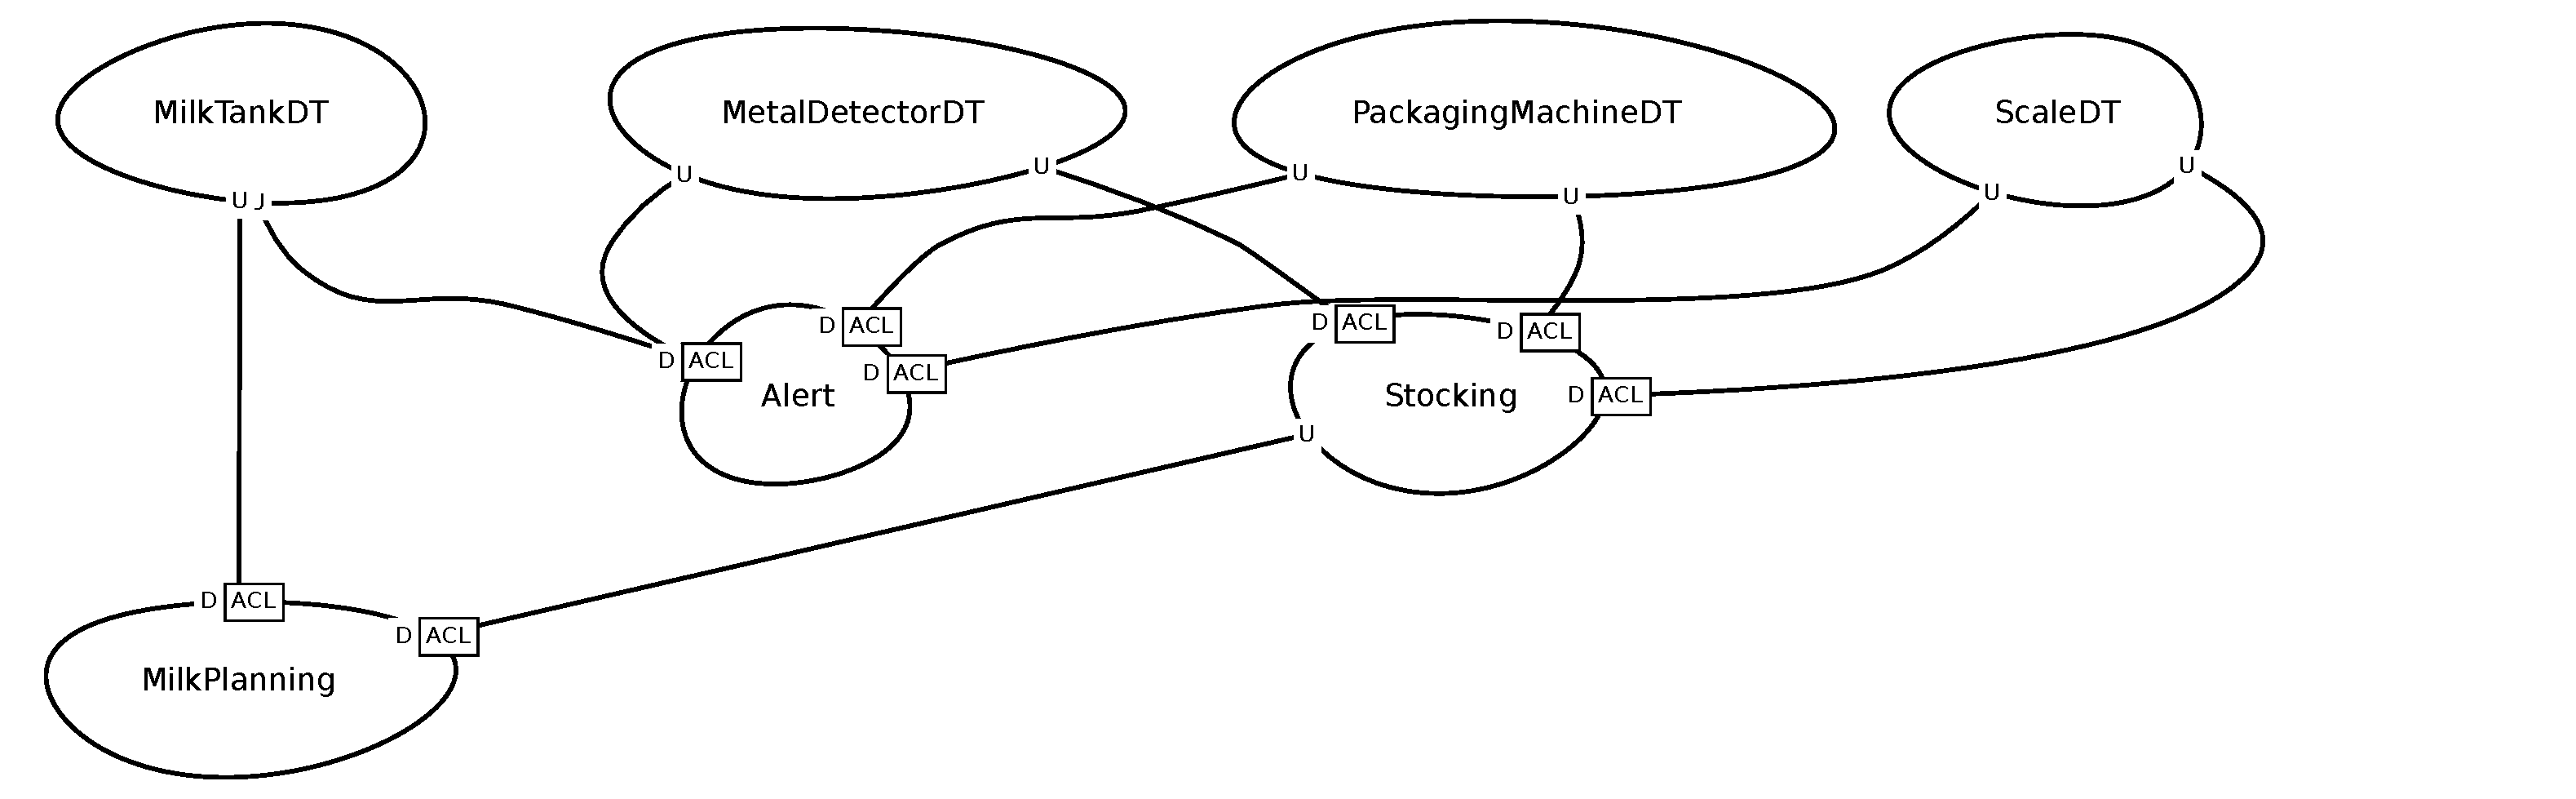
\includegraphics[width=\textwidth]{img/contextMap.eps}
    \caption{Context Map}
    \label{img:context-map}
\end{figure}


